\documentclass[conference]{IEEEtran}
\IEEEoverridecommandlockouts
% The preceding line is only needed to identify funding in the first footnote. If that is unneeded, please comment it out.
\usepackage{cite}
\usepackage{amsmath,amssymb,amsfonts}
\usepackage{algorithmic}
\usepackage{graphicx}
\usepackage{textcomp}
\usepackage{xcolor}
\usepackage{array,etoolbox,multirow}
\usepackage{float}


\def\BibTeX{{\rm B\kern-.05em{\sc i\kern-.025em b}\kern-.08em
    T\kern-.1667em\lower.7ex\hbox{E}\kern-.125emX}}
\begin{document}

\title{Conference Paper Title*\\
{\footnotesize \textsuperscript{*}Note: Sub-titles are not captured in Xplore and
should not be used}
\thanks{Identify applicable funding agency here. If none, delete this.}
}

\author{\IEEEauthorblockN{1\textsuperscript{st} Given Name Surname}
\IEEEauthorblockA{\textit{dept. name of organization (of Aff.)} \\
\textit{name of organization (of Aff.)}\\
City, Country \\
email address or ORCID}
\and
\IEEEauthorblockN{2\textsuperscript{nd} Given Name Surname}
\IEEEauthorblockA{\textit{dept. name of organization (of Aff.)} \\
\textit{name of organization (of Aff.)}\\
City, Country \\
email address or ORCID}
\and
\IEEEauthorblockN{3\textsuperscript{rd} Given Name Surname}
\IEEEauthorblockA{\textit{dept. name of organization (of Aff.)} \\
\textit{name of organization (of Aff.)}\\
City, Country \\
email address or ORCID}
\and
\IEEEauthorblockN{4\textsuperscript{th} Given Name Surname}
\IEEEauthorblockA{\textit{dept. name of organization (of Aff.)} \\
\textit{name of organization (of Aff.)}\\
City, Country \\
email address or ORCID}
\and
\IEEEauthorblockN{5\textsuperscript{th} Given Name Surname}
\IEEEauthorblockA{\textit{dept. name of organization (of Aff.)} \\
\textit{name of organization (of Aff.)}\\
City, Country \\
email address or ORCID}
\and
\IEEEauthorblockN{6\textsuperscript{th} Given Name Surname}
\IEEEauthorblockA{\textit{dept. name of organization (of Aff.)} \\
\textit{name of organization (of Aff.)}\\
City, Country \\
email address or ORCID}
}

\maketitle

\begin{abstract}
This document is a model and instructions for \LaTeX.
This and the IEEEtran.cls file define the components of your paper [title, text, heads, etc.]. *CRITICAL: Do Not Use Symbols, Special Characters, Footnotes, 
or Math in Paper Title or Abstract.
\end{abstract}

\begin{IEEEkeywords}
component, formatting, style, styling, insert
\end{IEEEkeywords}

\section{Requirements Specification}

Precursor to theorizing about the potential of microservices patterns for big data systems, we need to define what we mean by big data systems and what are the requirements of these systems. System and software requirements come in different flavour and can range from a sketch on a napkin to formal (mathematical) specifications. Therefore, we first need to identify what kind of requirements is the most suitable for the purposes of this study. To answer this question, we first explored the body of evidence to understand the current classification of software requirements. 

There's been various attempts to defining and classifying software and systems requirements. For instance, Sommerville (\cite{sommerville2011software}) classified requirements into three levels of abstraction that are namely 1) user requirements, 2) system requirements and 3) design specifications. The author then mapped these requirements against user acceptance testing, integration testing and unit testing. While this could satisfy the requirements of this study, we opted for a a more general framework provided by Laplante (\cite{laplante2017requirements}). In Laplante's approach, requirements are categorized into three categories of 1) functional requirements, 2) non-functional requirements, and 3) domain requirements. 

Our objective is to define the high-level requirements of big data systems, thus we do not seek to explore 'non-functional' requirements. Non-functional requirements are emerged from the particularities of an environment, such as a banking sector and do not correlate to our study. Therefore, the type of requirements we are looking for is functional and domain requirements.

After clarifying the type of requirements, we then explored the body of evidence to realize the general requirements of big data systems. Indeed, the most discussed characteristics of big data systems are the popular 5Vs which are velocity, veracity, volume, Variety and Value (\cite{Demchenko2014}, \cite{Bughin2016}, \cite{Bahrami2015}, \cite{rad2017big}, \cite{Marz2015}, \cite{Chen2016a} ). Many researchers such as Nadal et al. (\cite{nadal2017software}) have underpinned their artifact development on these characteristics and requirements that emerge from them. 

In an extensive effort, NIST Big Data Public Working Group embarked on a large scale study to extract requirements from variety of application domains such as Healthcare and Life Sciences, Commercial, Energy, Government, and Defense. The result of this study was the formation of general requirements under seven categories. In another effort by Volk et al. (\cite{volk2020identifying}),9 use cases for big data projects are identified by collecting theories and use cases from the literature and categorizing them using a hierarchical clustering algorithm. Bashari et al. (\cite{bashari2016security}) focused on the security and privacy requirements of big data systems, Yu et al. presented the modern components of big data systems \cite{yu2019components}, Eridaputra et al. (\cite{eridaputra2014modeling}) created a generic model for big data requirements using goal oriented approaches, and Al-jaroodi et al. (\cite{al2016characteristics}) investigated general requirements to support big data software development. 

We've also studied the reference architectures developed for big data systems to understand general requirements. In one study, Ataei et al. (\cite{ataei2020big}) assessed the body of evidence and presented with a comprehensive list of big data reference architectures. This study helped us realized the spectrum of big data reference architectures, how they are designed and the general set of requirements.  

By analyzing these studies and by evaluating the design and requirement engineering required for big data reference architectures, we created a set of high-level requirements based on big data characteristics. We have then looked for a rigorous approach to present these requirements. There are numerous approaches used for requirement representation including informal, semiformal and formal methods. For the purposes of this study, we opted for an informal method because it's a well established method in the industry and academia (\cite{kassab2014state}). 

Our approach follows the guidelines explained in ISO/IEC/IEEE standard 29148 for representing functional requirements. Our requirement repesentation is organized in system modes, that is we explain the major components of the system and then describe the requirements. This approach is inspired by the requirement specification expressed for NASA WIRE (wide-field infrared explorer) system explained in \cite{laplante2017requirements}. We also taken inspiration from Software Engineering Body of Knowledge Version (\cite{abran2004software}).

Taking all into consideration, we categorized our requirements based on the major characteristics of big data, that is value, variety, velocity, veracity, and volume (\cite{ataei}), plus  . These requirements are as followings: 

\newcounter{magicrownumbers}
\newcommand\rownumber{\stepcounter{magicrownumbers}\arabic{magicrownumbers}}

\begin{center}
    \begin{table*}
    \renewcommand*{\arraystretch}{1.8}
    \begin{tabular}{ | m{1.2cm} | m{14cm} |}

        \hline

        Volume &

        Vol-1) System needs to support asynchronous, streaming, and batch processing to collect data from centralized, distributed, and cloud data sources, and sensors, instrument and other IOT devices 
        
        Vol-2) System needs to provide a scalable storage for massive data sets 
 
        \\

        \hline

        Velocity & 
        
        Vel-1) System needs to support slow, bursty, and high-throughput data transmission between data sources and computing clusters
        
        Vel-2) System needs to stream data to data consumers in a timely manner 

        Vel-3) System needs to able to ingest multiple, continuous, time varying data streams 

        Vel-4) System shall support fast search from streaming and processed data with high accuracy and relevancy 
        
        Vel-5) System should be able to process data in real-time or near real-time manner 
    
        \\ 

        \hline

        Variety & 

        Var-1) System needs to support data in various formats ranging from structured to semi-structured and unstructured graph, web, text, document, timed, spatial, multimedia, simulation, instrumental, and geo-spatial data. 

        Var-2) System needs to support aggregation, standardization, and normalization of data from disparate sources 

        Var-3) System shall support adaptations mechanisms for schema evolution.

        Var-4) System can provide mechanisms to automatically include new data sources 

        \\

        \hline

        Value & 
        
        Val-1) System needs to able to handle compute-intensive analytical processing and machine learning techniques 
        
        Val-2) System needs to support two types of analytical processing: batch and streaming. 

        Val-3) System needs to support different output file formats for different purposes such as descriptive analytics, predictive analytics, reporting and visualizations. 
        
        Val-4) System needs to support streaming results to the consumers 

        \\

        \hline

        Security \& Privacy & 
        
        SaP-1) System needs to protect and retain privacy and security of sensitive data.

        SaP-2) System needs to have access control, and multi-level, policy-driven authentication on protected data and processing nodes. 

        \\

        \hline
        
        Veracity &
        
        Ver-1) System needs to support data quality curation including classification, pre-processing, format, reduction, and  transformation. 
        
        Ver-2) System needs to support data provenance including data life cycle management and long-term preservation.
        
        Ver-3) System needs to support data validation in two ways: automatic and human annotated. 

        Ver-4) System should be able to handle data loss or corruption. 
        
        \\

        \hline
  
    \end{tabular}
    \end{table*}
\end{center}


\section{Microservice Patterns}

As a result of this SLR, 50 microservice patterns have bene found. These patterns are then classified based on their function and the problem they solve. Each classifications and it's reasoning is depicted in table \ref{MS-Pattern-Cat}.


\begin{enumerate}
    \item Database per service \checkmark
    \item Shared database \checkmark
    \item Event sourcing \checkmark
    \item Multiple service instances per host \checkmark
    \item API gateway \checkmark
    \item Self registration \checkmark
    \item Service discovery \checkmark
    \item Circuit breaker \checkmark
    \item Bulkhead pattern \checkmark
    \item Command and query responsibility segregation \checkmark
    \item Competing consumers \checkmark
    \item Pipes and filters \checkmark
    \item Strangler \checkmark
    \item Anti-corruption layer \checkmark
    \item External configuration store  \checkmark
    \item Priority queue \checkmark
    \item Log Aggregation \checkmark
    \item Ambassador \checkmark
    \item Sidecar \checkmark
    \item Gateway aggregate \checkmark
    \item Gateway offloading \checkmark
    \item Aggregator \checkmark
    \item Backend for Frontend \checkmark
    \item API Composition \checkmark
    \item Saga transaction management \checkmark
    \item Static content hosting \checkmark
    \item Computer resource consolidation \checkmark
    \item Leader election \checkmark
  \end{enumerate}


  
\begin{center}
    \begin{table*}
    \renewcommand*{\arraystretch}{1.8}
    \begin{tabular}{ | m{3cm} | m{12cm} | }

        \hline

        Category &  Pattern
 
        \\

        \hline

        Data Management &  Database per Service, Shared Database, Event Sourcing, Command and Query Responsibility Segregation
 
        \\

        \hline

        Platform and Infrastructure & Multiple service instances per host, External configuration store, Sidecar, Static content hosting, Computer resource consolidation
 
        \\

        \hline

        Communicational & API gateway,  Anti-corruption layer, Self Registration, Service Discovery, Competing consumers, Pipes and filters, Priority queue, Ambassador, Gateway aggregate, Gateway offloading, Aggregator, Backend for Frontend, API Composition, Saga transaction management, Gateway routing, Leader election
        
 
        \\

        \hline

        Fault Tolerance & Circuit breaker, Bulkhead pattern
 
        \\
        \hline

        Observability & Log Aggregation Pattern
 
        \\
        \hline


    \end{tabular}
    \end{table*}
\end{center}



\begin{center}
    \begin{table*}
    \renewcommand*{\arraystretch}{1.8}
    \begin{tabular}{ | m{2cm} | m{8cm} |  m{2cm} |}

        \hline

        Requirement &  Patterns & Reasoning
 
        \\
        \hline

        Vol-1 &  
        
        1) Database per Service

        2)  Event Sourcing
        
        3)  Command and Query Responsibility Segregation
        
        4)  External Configuration Store
        
        5)  API gateway
        
        6)  Anti-Corruption Layer
        
        7)  Service Discovery
        
        8)  Self Registration
        
        9)  Priority Queue

        10) Gateway Offloading 

        11) Gateway Aggregate 

        12) Leader Election

        13) Log Aggregation Pattern 
        
        & Reasoning 
 
        \\

        \hline

        Vol-2 &  
        
        1) Database per Service  
        
        2) Command and Query Responsibility Segregation
        
        & Reasoning
        
        \\
        \hline

        Vel-1 &  
    
        1) API Gateway 

        2) Service Discovery 

        3) Pipes and Filters 

        4) Leader Election 

        5) Circuit Breaker 

        6) Log Aggregation  
        
        & Reasoning
        
        \\
        \hline

        Vel-2 &  
    
        1) Command and Query Responsibility Segregation
        
        2) API gateway

        3) Competing consumers

        4) Gateway aggregate

        5) Gateway Offloading

        6) Leader Election 

        & Reasoning

        \\

        \hline

        Vel-3 &  
    
        1) Command and Query Responsibility Segregation
        
        2) API gateway

        3) Competing consumers

        4) Gateway aggregate

        5) Gateway Offloading

        6) Leader Election 

        & Reasoning
        
        \\
        \hline

        \hline

        Vel-3 &  

        1) API composition
        
        2) API gateway

        4) Gateway aggregate

        5) Gateway Offloading

        & Reasoning
        
        \\
        \hline

        Vel-4 &  

        1) API composition
        
        2) API gateway

        4) Gateway aggregate

        5) Gateway Offloading
                
        6) Event Sourcing

        7) Command and Query Responsibility Segregation

        & Reasoning
        
        \\
        \hline

        Vel-5 &  

        1) Leader Election 

        2) Log Aggregation Pattern 

        & Reasoning
        
        \\
        \hline

        
        Var-1 &  
        
        None

        & Reasoning
        
        \\
        \hline

        Var-2 &  
        
        1)  Database per Service

        2) API Gateway

        & Reasoning
        
        \\
        \hline

        Var-3 & None  & Reasoning
        
        \\
        \hline

        Var-4 &  

        1) API Gateway

        2) Gateway Offloading

        3) Gateway Aggregate
        
        & Reasoning
        
        \\
        \hline
  
    \end{tabular}
    \end{table*}
\end{center}



\begin{center}
    \begin{table*}
    \renewcommand*{\arraystretch}{1.8}
    \begin{tabular}{ | m{2cm} | m{8cm} |  m{2cm} |}
        \hline

        Val-1 &  

        1) Event Sourcing

        2) Command and Query Responsibility Segregation

        3) Priority Queue

        4) Leader Election

        5) Bulkhead Pattern
        
        &  Reasoning 
        
        \\
        \hline

        Val-2 &  

        1) Event Sourcing

        2) Command and Query Responsibility Segregation

        3) API gateway, Gateway aggregate

        4) Gateway offloading

        5) Priority queue
        
        & Reasoning
        
        \\
        \hline

        Val-3 &  

        1) API gateway

        2) Anti-corruption layer

        3) Service Discovery

        4) Gateway aggregate

        5) Backend for Frontend
        
        & Reasoning
        
        \\
        \hline

        Val-4 &  

        1) Event Sourcing

        2) Command and Query Responsibility Segregation

        3) Backend for Frontend

        & Reasoning
        
        \\
        \hline

        SaP-1 &  

        1) External Configuration Store

        2) API Gateway

        3) Gateway Aggregate

        4) Backend for Frontend 
        
        & Reasoning
        
        \\
        \hline

        SaP-2 &  

        1) External Configuration Store

        2) API Gateway

        3) Gateway Aggregate

        4) Backend for Frontend 
        
        & Reasoning
        
        \\
        \hline

        Ver-1 &  

        1) Pipes and filters
        
        & Reasoning
        
        \\
        \hline

        Ver-2 &  
        None 
        & Reasoning
        
        \\
        \hline

        
        Ver-3 &  
        
        None

        & Reasoning
        
        \\
        \hline

             
        Ver-4 &  
        
        1) Circuit Breaker

        & Reasoning
        
        \\
        \hline

    \end{tabular}
    \end{table*}
\end{center}


\section{Application of Microservices Design Patterns to Big Data Systems}

In this section, we combine our findings from both SLRs, and present new theories on application of microservices design patterns for big data systems. The patterns gleaned, are established theories that are derived from actual problems in microservices systems in practice, thus we do not aim to re-validate them in this study. Moreover, we do not aim to validate the theories proposed in this study through an empirical study.

The main contribution of our work is to propose new theories and try to apply some of the well-known software engineering patterns to the realm of data engineering and in specific, big data. Based on this, we map big data system requirements against a pattern and provide with reasoning on why such pattern might work for big data systems. 

These descriptions are presented as sub section each describing one characteristic of big data systems. 


\subsection{Volume}

There has been two requirements associated to the Volume aspect of big data systems which are about the application handling various data types (Vol-1) and the application providing with a scalable storage (Vol-2). 

For Vol-1 and Vol-2 we suggest the following patterns to be effective: 

\begin{enumerate}
    \item External Configuration Store
    \item API gateway 
    \item Gateway offloading 
\end{enumerate}

Big data systems and microservices architecture are both inherently distributed. While majority of current big data applications are designed underlying a monolithic data pipeline architecture, here, we propose microservices architecture for a domain-driven and decentralized big data architecture. We support our arguments by the means of modeling. We use Archimate (\cite{lankhorst2013language}) as recommend in ISO/IEC/IEEE 42010 (\cite{Chaabane}). 

We posit that a pattern alone would not be significantly useful to a data engineering or a data architect, and propose that collection of a pattern in relation to current defacto standard of BD architectures is a better means of communication. 

To achieve this, we've portray patterns selected for each requirement in a reference architecture. We then justify the components and describe how patterns could address the requirement. For this purpose we portray the patterns for Vol-1 in figure \ref{fig-vol-1}


\begin{figure*}[h!]
    \centering 
    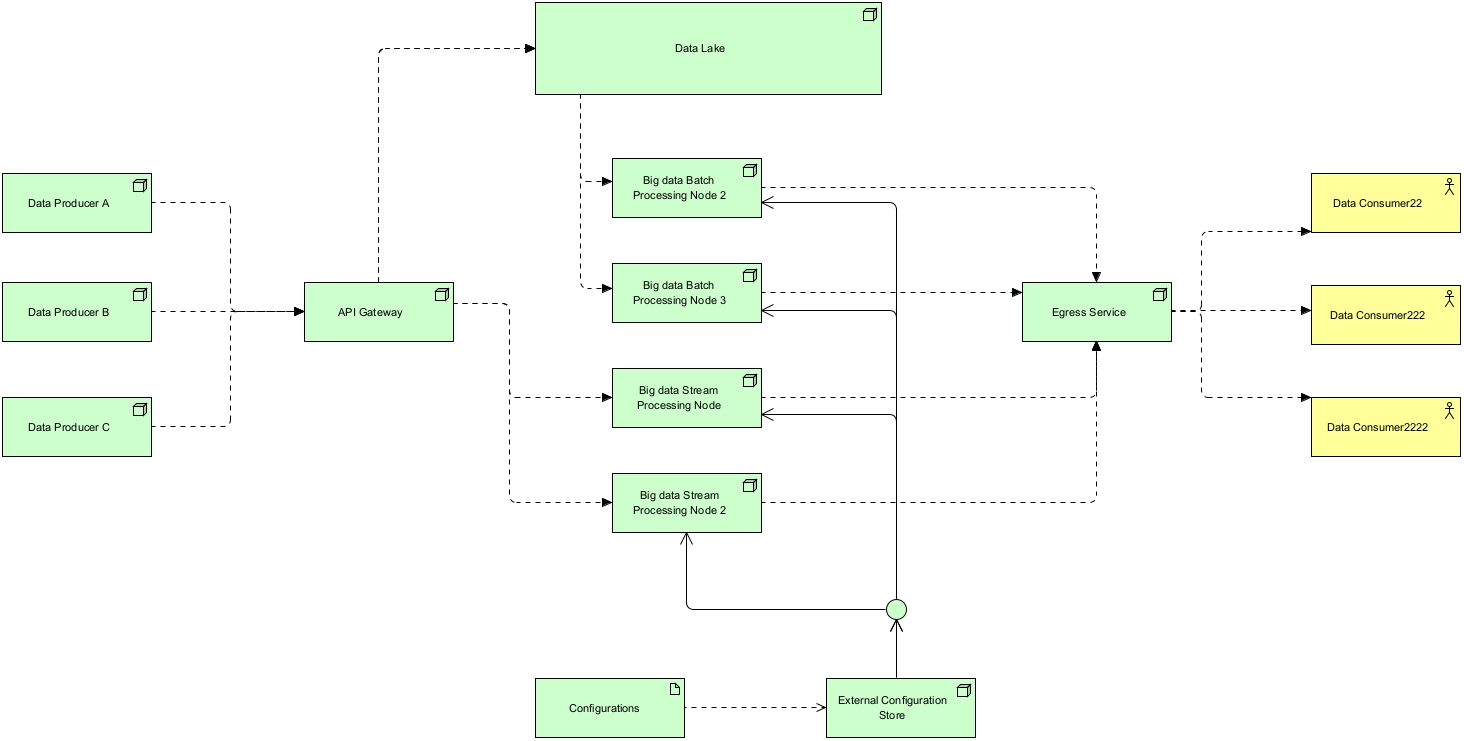
\includegraphics[width=17cm]{../Media/Vol-1 Requirement RA.jpg}
    \label{fig-vol-1}
    \caption{Design patterns for volume requirement}
\end{figure*}

\subsubsection{Gateway Offloading and API Gateway}

In a typical flow of data engineering, data goes from ingestion, to storage, to transformation and finally to serving. However there are various challenges to achieve this process. One challenge in this process is the realization of various data sources as described in Vol-1. The problem is that data comes in various formats from structured to semi-structured to unstructured, and the systems needs to handle different data through different interfaces. There is also streaming data that needs to be handled separately with different architectural constructs and data types. So some of the key engineering consideration for the ingestion process is that; 1) what are the typical use cases for the data being ingested ? is the big data system ingesting data reliably ? what is the next data destination ? How frequently should data be ingested ? In what volume the data typically arrives? Does streaming data need to be transformed before reaching the destination ? 

Given the challenges and particularities of data types, different nodes maybe spawned to handle the volume of data as witnessed in big data reference architectures studied by Ataei et al (\cite{ataei2020big}). Another popular approach is the segregation of concerns by separating batch and streaming processing nodes. Given the requirement of horizontal scaling for big data systems, it is safe to assume that there is usually more then one node associated to the data being ingested. This can be problematic as different nodes will need to account for security, privacy and overall regulations of the context, alongside, the software engineering demand that each may have. 

This means that each node needs to reimplement the same interface for the aforementioned cross-cutting concerns, which makes scalability and maintainability of the big data system a daunting task. This also introduces unnecessary repetition of codes. To solve this problem, we explore the concept of gateway offloading and API gateway patterns. By offloading cross-cutting concerns that are shared across nodes to a single architectural construct, the API gateway in this case, not only we will achieve a separation of concerns and a good level of usability, but we increase security and performance, by processing and filtering incoming data through a well specified ingress. 

Moreover, if data producers directly communicate with the processing nodes, they will have to update the endpoint address every now and on. This issue is exacerbated when the service tries to communicate with a service that is down. Given that, the lifecycle of a service in a typical distributed cloud environment is not deterministic and many container orchestration systems constantly recycle services to proactively address this issue, reliability and maintainability of the big data system can be compromised. This scenario remains the same, and can be even worst if the company decides to have an on-premise data center. 

Additionally, the gateway can increase the system reliability and availability by doing a constant health check on services, and distribute traffic based on healthy nodes. The is also an array of other benefits such as having a weighted distribution, and creating a special cache mechanism through specific HTTP headers. This also means that if the gateway is down, service nodes won't introduce bad data or state into the overall system. We have portrayed a very simplistic representation of this pattern in fig \ref{fig-vol-1}. 

\subsubsection{External Configuration Store}

As discussed earlier, big data systems are made up of various nodes in order to achieve horizontal scalability. While these systems are logically separated to their own service, they will have to communicate with each other in order to achieve the goal of the system. Thus each one of them will require a set of runtime environmental configuration to achieve their functionality. These configurations could be database network locations, feature flags, and third party credentials. Moreover, different stages of the data engineering may have different environments for different purposes, for instance, privacy engineers may require a completely different environment to achieve their requirements. 

Thus, the challenge is the management of these configurations as the system scale, and enabling services to run in different environments without modification. To address this problem, we propose the external configuration store pattern, also known as the 'externalized configuration pattern'. By externalizing all nodes configuration to another service, each node can request its configuration from an external store on boot up. This can be achieved in Docker files through the CMD command, or could be written in Terraform codes for a Kubernetes pod. This pattern is portrayed in fig \ref{fig-vol-1}.

\subsection{Velocity}

Velocity is perhaps one of the most challenging aspects of the big data systems, which if is not architected well, can result in series of issues from system availability to massive loses and customer churn. 

To address some of the challenges associated with the velocity aspect of big data systems, we recommend the following patterns for the requirements Vel-1, Vel-2, Vel-3, and Vel-5: 

\begin{enumerate}
    \item Competing Consumers
    \item Circuit Breaker
    \item Log Aggregation
\end{enumerate}

\subsubsection{Competing Consumers}

Big data doesn't imply only 'big' or a lot of data, it also implies the rate at which data can be ingested, stored and analyzed to produce insights. According to a recent MIT report in collaboration with Databricks, one of the main challenges of big data 'low-achievers' is the 'slow processing of large amounts of data'. If the business desires to go data driven, it should be able to have time-to-insight within an acceptable range, as the decisions have to be made at the end of the day. 

Achieving this in such a distribute setup as big data systems with so many moving parts, is a challenging task, but there are microservices pattern that can be tailored to help with some of these challenges. Given the very contrived scenario of a big data system described in the previous section, at the very core, data needs to be ingested quickly, stored in a timely manner, micro-batch, batch, or stream processed, and lately served to the consumers. So what happens if one node goes down or becomes unavailable? in a traditional Hadoop setup, if Mesos is utilized as the scheduler, the node will be restarted and will go through a lifecycle again. 

This means during this period of time, the node is unavailable, and any workload for stream processing has to wait, failing to achieve requirements Vel-2, Vel-3 and Vel-5. This issue is exacerbated if the system is designed and architected underlying monolithic pipeline architecture with point-to-point communication. One way to solve some of these issues is to introduce an event driven communication as portrayed in the works of Ataei et al (\cite{ataei2021neomycelia}), and try to increase fault tolerance and availability through competing consumers, circuit breaker, and log aggregation. 

Underlying the event-driven approach, we can assume that nodes are sending each other events as a means of communication. This implies that node A can send an event to node B in a 'dispatch and forget' fashion on a certain topic. However this pattern introduces to same problem as the point-to-point REST communication style, as if node B is down, then this will have a ripple effect on data engineering pipelines. To address this challenge, we can adopt the competing consumer pattern. Adopting this pattern means instead of one node listening on the topic, there will be a few nodes. This can change the nature of the communication to asynchronous mode, and allow for a better fault tolerance, because if one node is down, the other nodes can listen to the event and handle it. This will help alleviate challenges in regards to Vel-2, Vel-3 and Vel-5.

\subsubsection{Circuit Breaker}

On the other hand, given the large number of nodes one can assume for any big data system, one can employ the circuit breaker pattern to signal the service unavailability. Circuit breakers can protect the overall integrity of data and processes by tripping and closing the incoming request to the service. This communicates effectively to the rest of the system that the node is unavailable and a compelling decision can be made. This mixed with competing consumers pattern con increase the overall availability and reliability of the system, by providing an even-driven asynchronous fault tolerance communication mechanism. This allows system to be able to be resilient and responsive to bursty, high-throughput data as well as small, batch oriented data, addressing requirements Vel-1, Vel-4, and Vel-5. 
    
\subsection{Log Aggregator}

Along the lines log aggregation can be implemented to shed lights on various services and their audit trail. Traditional service based logging does not work very well in distributed environments, as engineers are required to understand the whole flow of data from one end to another. To address this issue, log aggregation can be implemented, which usually comes with an unified interface that services communicates to and log their processes. This interface then does the necessary mutations, store the logs. In addition, reliability engineers can configure alerts to be triggered underlying certain conditions. This increases teams agility to proactively resolve issue, which in turn increases reliability and availability which in turn addresses the velocity requirement of big data systems. While this design pattern does not directly affect any system requirements, it indirectly affects all of them.


A simplistic reference architecture of these patterns have been portrayed in fig \ref{fig-vel-ra}


\begin{figure*}[h!]
    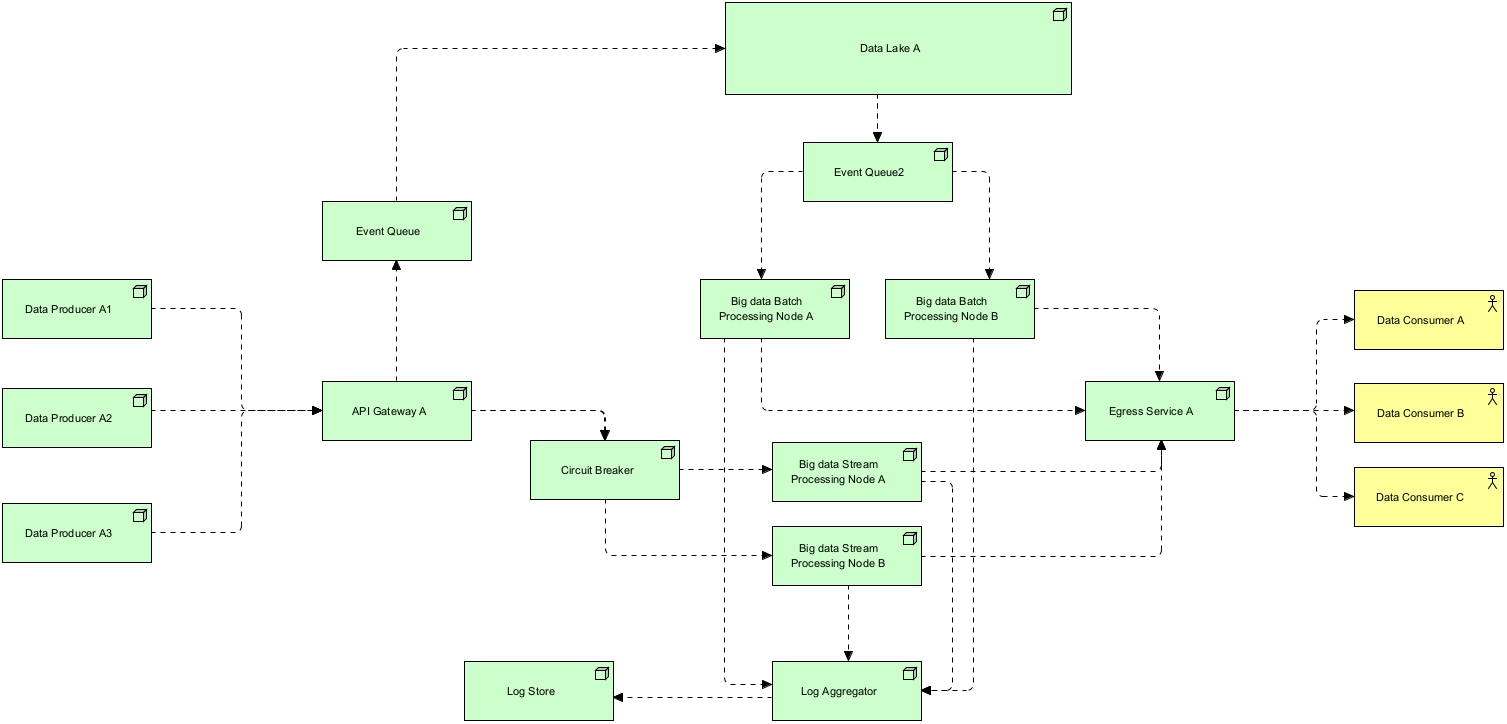
\includegraphics[width=17cm]{../Media/Velocity Requirement.jpg}
    \caption{Design patterns for velocity requirement}
    \label{fig-vel-ra}
\end{figure*}


\subsection{Variety}

Variety, being another important aspect of big data, implies the range of different data types and th challenges of handling these data. As more and more softwares become ubiquitous, newer data structures emerge, and an effective big data system must be elastic enough to handle various data types. 

To address some of the challenges of this endeavour, we recommend the following patterns to address requirements Var-1, Var-3, Var-4: 

\begin{enumerate}
    \item API Gateway 
    \item Gateway Offloading
\end{enumerate}

\subsubsection{API Gateway and Gateway Offloading}

We have previously discussed the benefits of API Gateway and Gateway Offloading, however in this section we aim to relate it more to big data system requirements Var-1, Var-3, and Var-4. API gateway is a great architectural construct to allow for rapid change of nodes that handle streaming and batch oriented workloads. Data engineers need to keep an open line of communication to data producers on change that could break the data pipelines and analytics. Suppose that developer A changes a field in a schema of an object that may break a pipeline or introduce a privacy threat. How can data engineers handle this scenario effectively? 

To address this problem, and to address big data requirements Var-1, Var-3, and Var-4, API Gateway and Gateway Offloading can be used. API Gateway and Gateway Offloading could be good patterns to offload some of the light weight processes that may associated to the data structure or the type of data. For instance, a light weight metadata check or data scrubbing can be achieved in the Gateway. However, Gateways themselves should be taking a lot of responsibility and possess a bottleneck to the system. Thus as nodes increase and requirements emerge, one might chose to opt for 'Backend for Frontend' pattern.

We do not do any modeling for this section, as the high-level overview of API Gateway pattern is portrayed in fig \ref{fig-vol-1}.

\subsection{Value}

Value is the nucleus of any big data endeavour. In fact all components of the system pursue the goal of realizing a value, that is the insight derived from the data. Howbeit, realizing these insights require a complex engineering. 

To address some of these challenges, we propose the following patterns to address the requirements Val-1, Val-3, and Val-4

\begin{enumerate}
    \item Command and Query Responsibility Segregation (CQRS)
    \item Anti-Corruption Layer 
    \item Gateway Offloading 
\end{enumerate}

\subsubsection{Command and Query Responsibility Segregation}

Suppose that there are various application that would like to query data in different ways and with different frequencies (Val-3, Val-4). Different consumers such as business analysts and machine learning engineers have very different demands, and would therefore create different workloads for the big data systems. As the consumers grow, the application has to handle more object mappings and mutations to meet the consumers demands. This may result in complex validation logics, mutations, and serialization that can be write-heavy on the data storage. As a result the serving layer can end up with an overly complex layer that does too much. 

Read and write workloads are really different, and this is something a data engineering should consider from the initial data modeling, to data storage, retrieval and potential serialization (JSon to Parquet). And while the system may be more tolerant on the write side, it may have a requirement to provide reads in a timely manner (checking a fraudulent credit card). Moreover, read and write representation of the data are often different and miss-matching and managing security and privacy can become complicated. 

To address some of this challenges, we presented event sourcing and command, CQRS. CQRS separates the read from writes, using commands to update the data, and query to read data. This implies that the read and write database can be physically segregated and consistency can be achieved through an event. To keep databases in sync, the write database can publish an event whenever an update occurs, and the read database can listen to it and update its values. This allows for elastic scaling of the read nodes, and allow for an increased query performance, especially in big data systems that have got egress services sitting on an edge. Therefore, this pattern can potentially address the requirement Val-1, and Val-3. 

\subsubsection{Anti-Corruption Layer}

Another pattern that comes useful when handling large number of data consumers is the anti-corruption layer. Given that the number of consumers and producers can grow and data can be created and requested in different formats with different characteristics, the ingestion and serving layer may be coupled to these foreign domains and try to account for an abstraction that aims to encapsulate all the logic in regards to all the external nodes. As the system grows, this abstraction layer becomes harder to maintain, and its maintainability attribute diminishes. 

One approach to solve this issue is anti-corruption layer. Anti-corruption layer is a node that is placed between the serving layer and data consumers, isolating different systems and translating communication. This eliminates all the complexity and coupling that could have been otherwise introduced to the serving layer. This also allows for nodes to follow the 'single responsibility' pattern (\cite{gamma1995design}). Anti-corruption layer can define strong interfaces and quickly serve new demands without affecting much of the serving node's abstraction. In another terms, it avoids corruption that may happen among systems, by separating them. This pattern can help with requirements Val-3 and Val-4. We have portrayed this pattern and CQRS in fig \ref{fig:Value Requirements}.

\subsubsection{Gateway Offloading}

We have previously discussed this pattern, but in this section we aim to relate more to the value requirements of BD. Given that the various nodes in the system may require services such as authentication, authorization, monitoring, logging, and throttling, it would become really difficult to address the value aspect of big data in a timely manner. To address these issues and to achieve Val-3 and Val-4, we recommend the gateway offloading pattern. Employing this pattern abstracts out cross-cutting services from each node and creates a unified interface that each node can utilize. This simplifies the development of new services for handling new data formats, and free data engineers from implementing features that requires special knowledge such as security and privacy. 

\begin{figure}[h]
    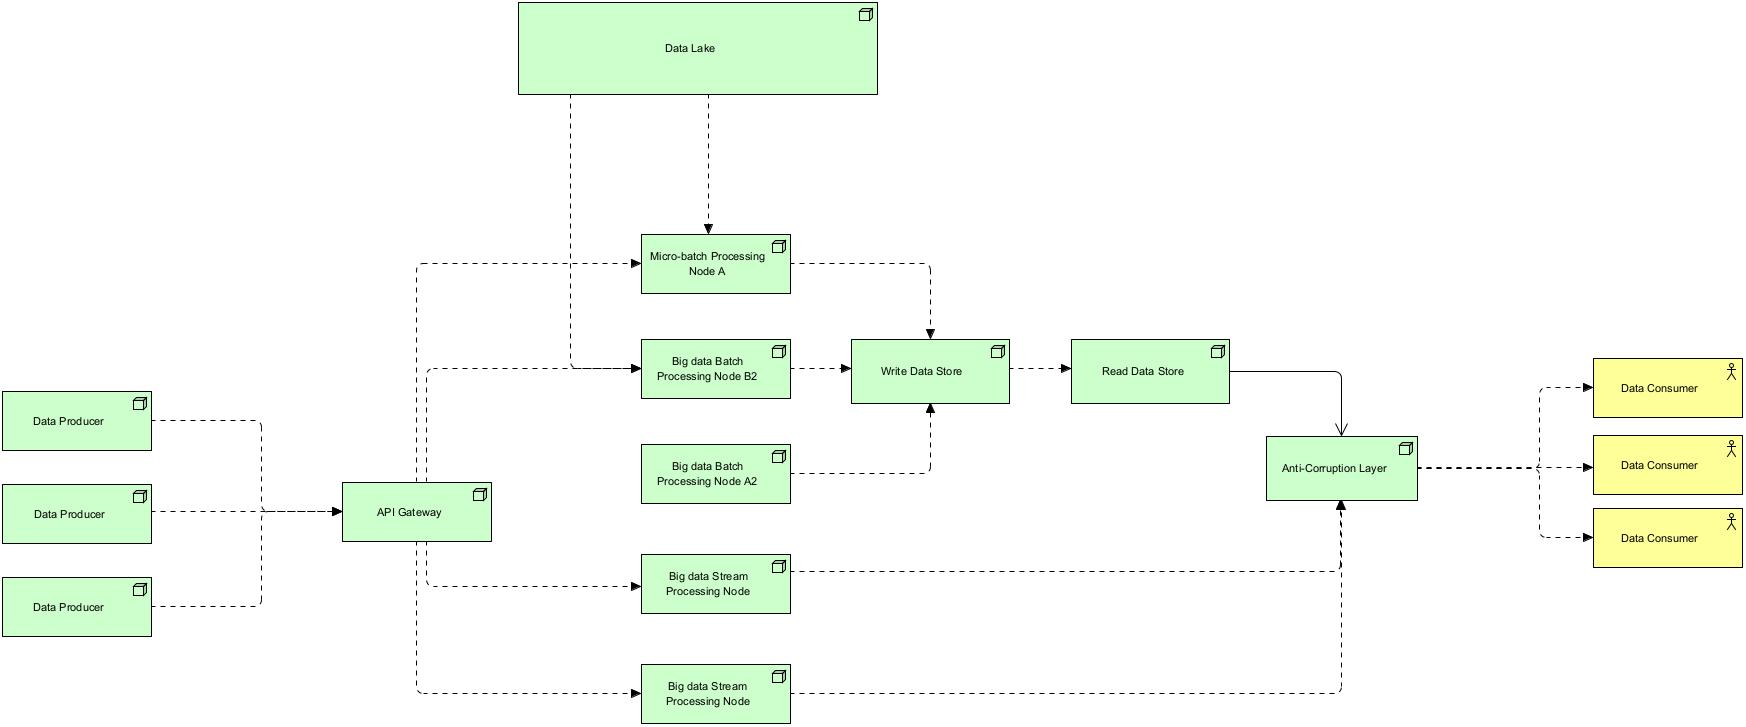
\includegraphics[width=17cm]{../Media/Value Requirement.jpg}
    \caption[]{Design patterns for value requirement }
    \label{fig:Value Requirements}
\end{figure}

\subsection{Security and Privacy}

Security and privacy should be on top of mind for any big data system development, as these two aspects play an important role in the overall data strategy and architecture of the company. At the intersection of data evolution, regional policies, and company policies, there's a great deal of complexity. To this end, we propose the following patterns to address requirements SaP-1 and SaP-2;

\begin{enumerate}
    \item Backend for Frontend (BFF)
\end{enumerate}

\subsubsection{BFF}

API gateway has been discussed in several sections in this study, however, in this section we are interested to see how it can improve security and privacy of big data systems. In terms of privacy, given the increasing load of data producers, and how they should be directed to the right processing node, how does one comply with regional policies such as GDPR? how do we ensure for example that data is anonymized and identifiable properties are omitted? one approach could be to do this right in the batch or stream processing nodes. However as data consumers grow and more data gets in, maintaining the privacy rules and applying them correctly to the dataset becomes more difficult. This becomes a perfect ground for mistake, and can potentially introduce legal issues to the company. 

On approach to this problem can be the BFF pattern. By creating backends (services) for frontends (data producers), we can logically segregate system's ingress for data that requires different level of privacy and security. This logical separation can include other factors such as QoS, key accounts, and even the nature of the API (GraphQL or RPC). Implementing this pattern means that instead of trying to account for all privacy related concerns in one node, we separate the concerns to a number of nodes that are each responsible for a specific requirement. This means, instead of creating a coupled, loosely abstracted implementation of privacy engineering, the system can benefit from hiding sensitive or unnecessary data before sending it to the up-stream node. This is also a great opportunity for data mutation, schema validation, and potentially protocol change (REST to Graph).

On the other hand, from the security point of view, and in specific in relation to authorization and authentication, this pattern provides with a considerable advantage. BFF can be implemented to achieve token isolation, cookie termination, and can serve as a security gate before requests can reach to upstream servers. Other security procedures such as sanitization, data masking, tokenization, and obfuscation can be done in this layer as well. As these BFF servers are logically isolated for specific requirements, maintainability and scalability is increased. This addresses the requirements SaP-1 and SaP-2. 


\subsection{Veracity}

Next to value, veracity is an integral component of any effective big data system. Veracity in general is about how truthful and reliable data is, and how signals can be separated from the noises. Data should conform with the expectations from the business, thus data quality should be engineered across the data lifecycle. According to Eryurek et al (\cite{eryurek2021data}), data quality can be defined by three main characteristics 1) accuracy, 2) completeness, and 3) timeliness. Each of these characteristics posit a certain level of challenge to architecture and engineering of big data systems. 

To this, we propose the following patterns for addressing requirements Ver-1, and Ver-4; 

\begin{enumerate}
    \item Pipes and Filters 
    \item Circuit breaker 
\end{enumerate}

\subsection{Pipes and Filters}

Suppose that there is a data processing and transformation node that is responsible for performing variety of data transformation and other processes with different level of complexities. As requirements emerge and newer, varying processing may be required, and soon this node will turn into a big monolithic unit that aims to achieve too much. Furthermore, this node is likely to reduce the opportunities optimization, refactoring, testing and reusing. In addition, as the business requirements emerge, the nature of some of these tasks may be different. Some processes may require a different metadata strategy that requires more computing resources, while others might not require such expensive resources. This is not elastic and can produce unwanted idle times. 

One approach to this problem could be the pipes and filters pattern. By implementing pipes and filters, processing required for each stream can be separated into its own node (filter) that performs a single task. This resembles to the well-known pattern of 'single responsibility' (\cite{gamma1995design}). Following this approach allows for standardization of the format of the data and processing required for each step. This can help avoiding code duplication, and results in easier removal, replacement, augmentation and customization of data processing pipelines, addressing the requirements Ver-1 and Ver-4.

\subsection{Circuit breaker}
 
In an inherently distributed environment like big data, calls to different services may fail due to various issues such as timeouts, transient faults or service being unavailable. While these faults maybe transient, this can have a ripple effect on other services in the system, causing a cascading failure across several nodes. This affects system availability and reliability and can cause major losses to the business. 

One solution to this problem can be the circuit breaker pattern. Circuit breaker is a pattern that prevents an application from from repeatedly trying to access a service that is not available. This improves the fault tolerance among services, and signals the service unavailability. The requesting application can decide accordingly on how to handle the situation. In other terms, circuit breakers are like proxies for operations that might fail. This proxy is usually implemented as a state machine having the states close, open, and half-open. Having this proxy in place provides stability to the overall big data system, when the service of interest is recovering from an incident. This can indirectly help with Ver-4.


\bibliographystyle{IEEEtran}
\bibliography{references}

\end{document}
        